%%%%%%%%%%%%%%%%%%%%%%%%%%%%%%%%%%%%%%%%%%%%%%%%%%%%%%%%%%%%%%%%%%%%%%
% How to use writeLaTeX: 
%
% You edit the source code here on the left, and the preview on the
% right shows you the result within a few seconds.
%
% Bookmark this page and share the URL with your co-authors. They can
% edit at the same time!
%
% You can upload figures, bibliographies, custom classes and
% styles using the files menu.
%
%%%%%%%%%%%%%%%%%%%%%%%%%%%%%%%%%%%%%%%%%%%%%%%%%%%%%%%%%%%%%%%%%%%%%%

\documentclass[12pt]{article}

\usepackage{sbc-template}

\usepackage{graphicx,url}

\usepackage[brazil]{babel}
\usepackage[utf8]{inputenc}
\usepackage{float}

\sloppy

\title{Análise de Desempenho Paralelo de Modelos de Difusão de Contaminantes em
  Água}

\author{Eduardo Verissimo Faccio, Pedro Figueiredo Dias, \\
  Pedro Henrique de Oliveira Masteguin}

\address{Instituto de Ciência e Tecnologia -- Universidade Federal de São Paulo
  (UNIFESP)\\
  São José dos Campos -- SP -- Brasil
  \email{\{verissimo.eduardo,pedro.figueiredo,p.masteguin\}@unifesp.br}
}

\begin{document}

\maketitle

% \begin{resumo} 
%   Este meta-artigo descreve o estilo a ser usado na confecção de artigos e
%   resumos de artigos para publicação nos anais das conferências organizadas
%   pela SBC. É solicitada a escrita de resumo e abstract apenas para os artigos
%   escritos em português. Artigos em inglês deverão apresentar apenas abstract.
%   Nos dois casos, o autor deve tomar cuidado para que o resumo (e o abstract)
%   não ultrapassem 10 linhas cada, sendo que ambos devem estar na primeira
%   página do artigo.
% \end{resumo}

\section{Introdução}

A contaminação de corpos d'água, tais como lagos e rios, é um grande desafio ao
meio ambiente e a saúde pública, sendo preciso entender a dispersão do
contaminante no ambiente para poder realizar qualquer intervenção de mitigação.
Dessa forma, este trabalho foca na modelagem numérica da difusão de poluentes
em uma matriz bidimensional, utilizando o método de diferenças finitas para
aproximar a equação de difusão discreta:

\begin{equation}
  C_{i,j}^{t+1} = C_{i,j}^t + D \cdot \Delta t \cdot \left( \frac{C_{i+1,j}^t +
    C_{i-1,j}^t + C_{i,j+1}^t + C_{i,j-1}^t - 4 \cdot C_{i,j}^t}{\Delta x^2}
  \right)
  \label{eq:Difusao}
\end{equation}

Nesta equação, $C_{i,j}^t$ representa a concentração do contaminante na célula
$(i,j)$ no instante $t$, $D$ é o coeficiente de difusão, $\Delta t$ o intervalo
de tempo discreto e $\Delta x$ o espaçamento espacial. O objetivo principal é
desenvolver uma simulação que modele a difusão de contaminantes aplicando
programação paralela para acelerar os cálculos e analisar o comportamento dos
poluentes ao longo do tempo. Serão comparadas as versões sequencial e paralela
do algoritmo, utilizando OpenMP, CUDA e MPI para explorar o processamento
simultâneo em múltiplos núcleos e dispositivos. Os resultados serão validados
por meio de mapas de calor, gráficos de speedup e eficiência, além da
comparação das matrizes geradas. Este estudo demonstra como técnicas de
programação concorrente e distribuída podem otimizar simulações numéricas
complexas, reforçando os conceitos aprendidos na disciplina e demonstrando sua
aplicação prática no desenvolvimento de soluções eficientes.

\section{Implementação do Algorítimo}

\subsection{Código Sequencial}

O código sequencial implementa a solução numérica da equação de difusão usando
uma abordagem serial. Utilizando-se do método de diferenças finitas, é simulado
a dispersão de uma substância em uma matriz bidimensional. Cada célula da
matriz representa a concentração de uma substância em um ponto do espaço.

O cálculo é realizado em um laço de repetição que itera sobre todas as células
da matriz. A atualização de cada célula depende da média das concentrações dos
seus vizinhos imediatos e de parâmetros físicos como coeficiente de difusão, o
intervalo de tempo $\Delta t$ e o espaçamento espacial $\Delta x$.

\subsection{Código Paralelo em MPI}

A implementação do código foi desenvolvida utilizando MPI (Message Passing
Interface) e OpenMP para combinar processamento distribuído e paralelismo em
nível de threads. O objetivo principal do código é resolver uma equação
diferencial parcial em um grid bidimensional, distribuindo os cálculos entre
múltiplos processos MPI e utilizando OpenMP para paralelismo dentro de cada
processo.

O fluxo de execução consiste nas seguintes etapas:

\begin{itemize}
  \item \textbf{Inicialização:} Inicia com MPI\_Init\_thread(), definindo o número de processos e threads OpenMP. Cada processo MPI recebe sua parte da matriz global.
  \item \textbf{Troca de dados entre processo:} Os processos MPI trocam as fronteiras das suas submatrizes com processos vizinhos usando comunicação assíncrona (MPI\_Isend() e MPI\_Irecv()).
  \item \textbf{Calculo Paralelo:} Cada processo MPI aplica a equação diferencial na sua submatriz, paralelizando o cálculo com OpenMP (\#pragma omp parallel for).
  \item \textbf{Sincronização global:} A diferença entre os estados da matriz é calculada localmente e reduzida globalmente com MPI\_Allreduce(), garantindo consistência entre os processos.
  \item \textbf{Finalização:} Após completar todas as iterações, a memória é liberada e MPI\_Finalize() é chamado. O tempo total de execução é registrado e exibido pelo processo mestre.

\end{itemize}

Esse fluxo de execução garante que a carga de trabalho seja distribuída de
maneira eficiente entre os processos MPI, enquanto OpenMP melhora o desempenho
dentro de cada nó de processamento.

\subsection{Interface Python e ferramenta CMake}

O projeto utiliza o CMake como sistema de compilação para gerenciar processos e
dependências tanto da implementação em OpenMP quanto da versão CUDA, definindo
tudo por meio de arquivos de configuração. Para destacar as diferenças de
desempenho entre as abordagens sequencial, OpenMP e CUDA, as otimizações do
compilador — como a vetorização automática que inicialmente minimizava essas
disparidades — são desabilitadas por meio de flags específicas, permitindo uma
execução mais direta e comparável.

Paralelamente, foi implementada uma interface Python usando o módulo
\textit{ctypes} para carregar dinamicamente as bibliotecas compiladas e mapear
suas funções, facilitando a integração com métodos de análise e visualização
desenvolvidos em notebooks Jupyter. Inspirada em bibliotecas como o NumPy, essa
abordagem combina a eficiência das implementações em C com a flexibilidade e a
facilidade de uso do Python, possibilitando a configuração de parâmetros como
tamanho da matriz, coeficiente de difusão e dimensões dos blocos de
\textit{threads}.

\section{Resultados}

Nesta seção, apresentamos os resultados obtidos de nossa implementação.
Inicialmente, analisamos a equivalência lógica entre os códigos sequencial e
paralelo, considerando possíveis erros que podem surgir na paralelização, como
condições de corrida ou inconsistências de sincronização. Em seguida,
ilustramos, por meio de mapas de calor, a atualização dos valores da matriz ao
longo do tempo. Por fim, realizamos uma análise comparativa dos tempos médios
de execução e \textit{speedup} entre as duas versões.

\subsection{Validação da Implementação}

Para assegurar a correção das duas implementações, verificamos em cada iteração
se os valores presentes em cada célula da matriz são idênticos. Dessa forma, o
resultado na última iteração deve ser o mesmo em ambas as versões.

Por meio desse procedimento, utilizando a interface Python em conjunto com um
Jupyter Notebook, comprovamos que as duas soluções produzem resultados
idênticos. Isso era esperado, pois no código paralelo não ocorrem condições de
corrida, uma vez que a escrita não é realizada na mesma região de memória das
leituras, tornando o processamento de cada célula pelas \textit{threads}
independente.

\subsection{Validação da Implementação}

Para ilustrar o funcionamento da implementação, foram gerados mapas de calor,
representado pela Figura \ref{fig:heatmap}, nos quais cada ponto de uma matriz
50x50 é representado por uma cor distinta. Cores escuras correspondem a valores
próximos de um, indicando alta concentração do contaminante, enquanto cores
claras representam valores próximos de zero, indicando baixa presença de
contaminação.

\begin{figure}[ht]
  \centering
  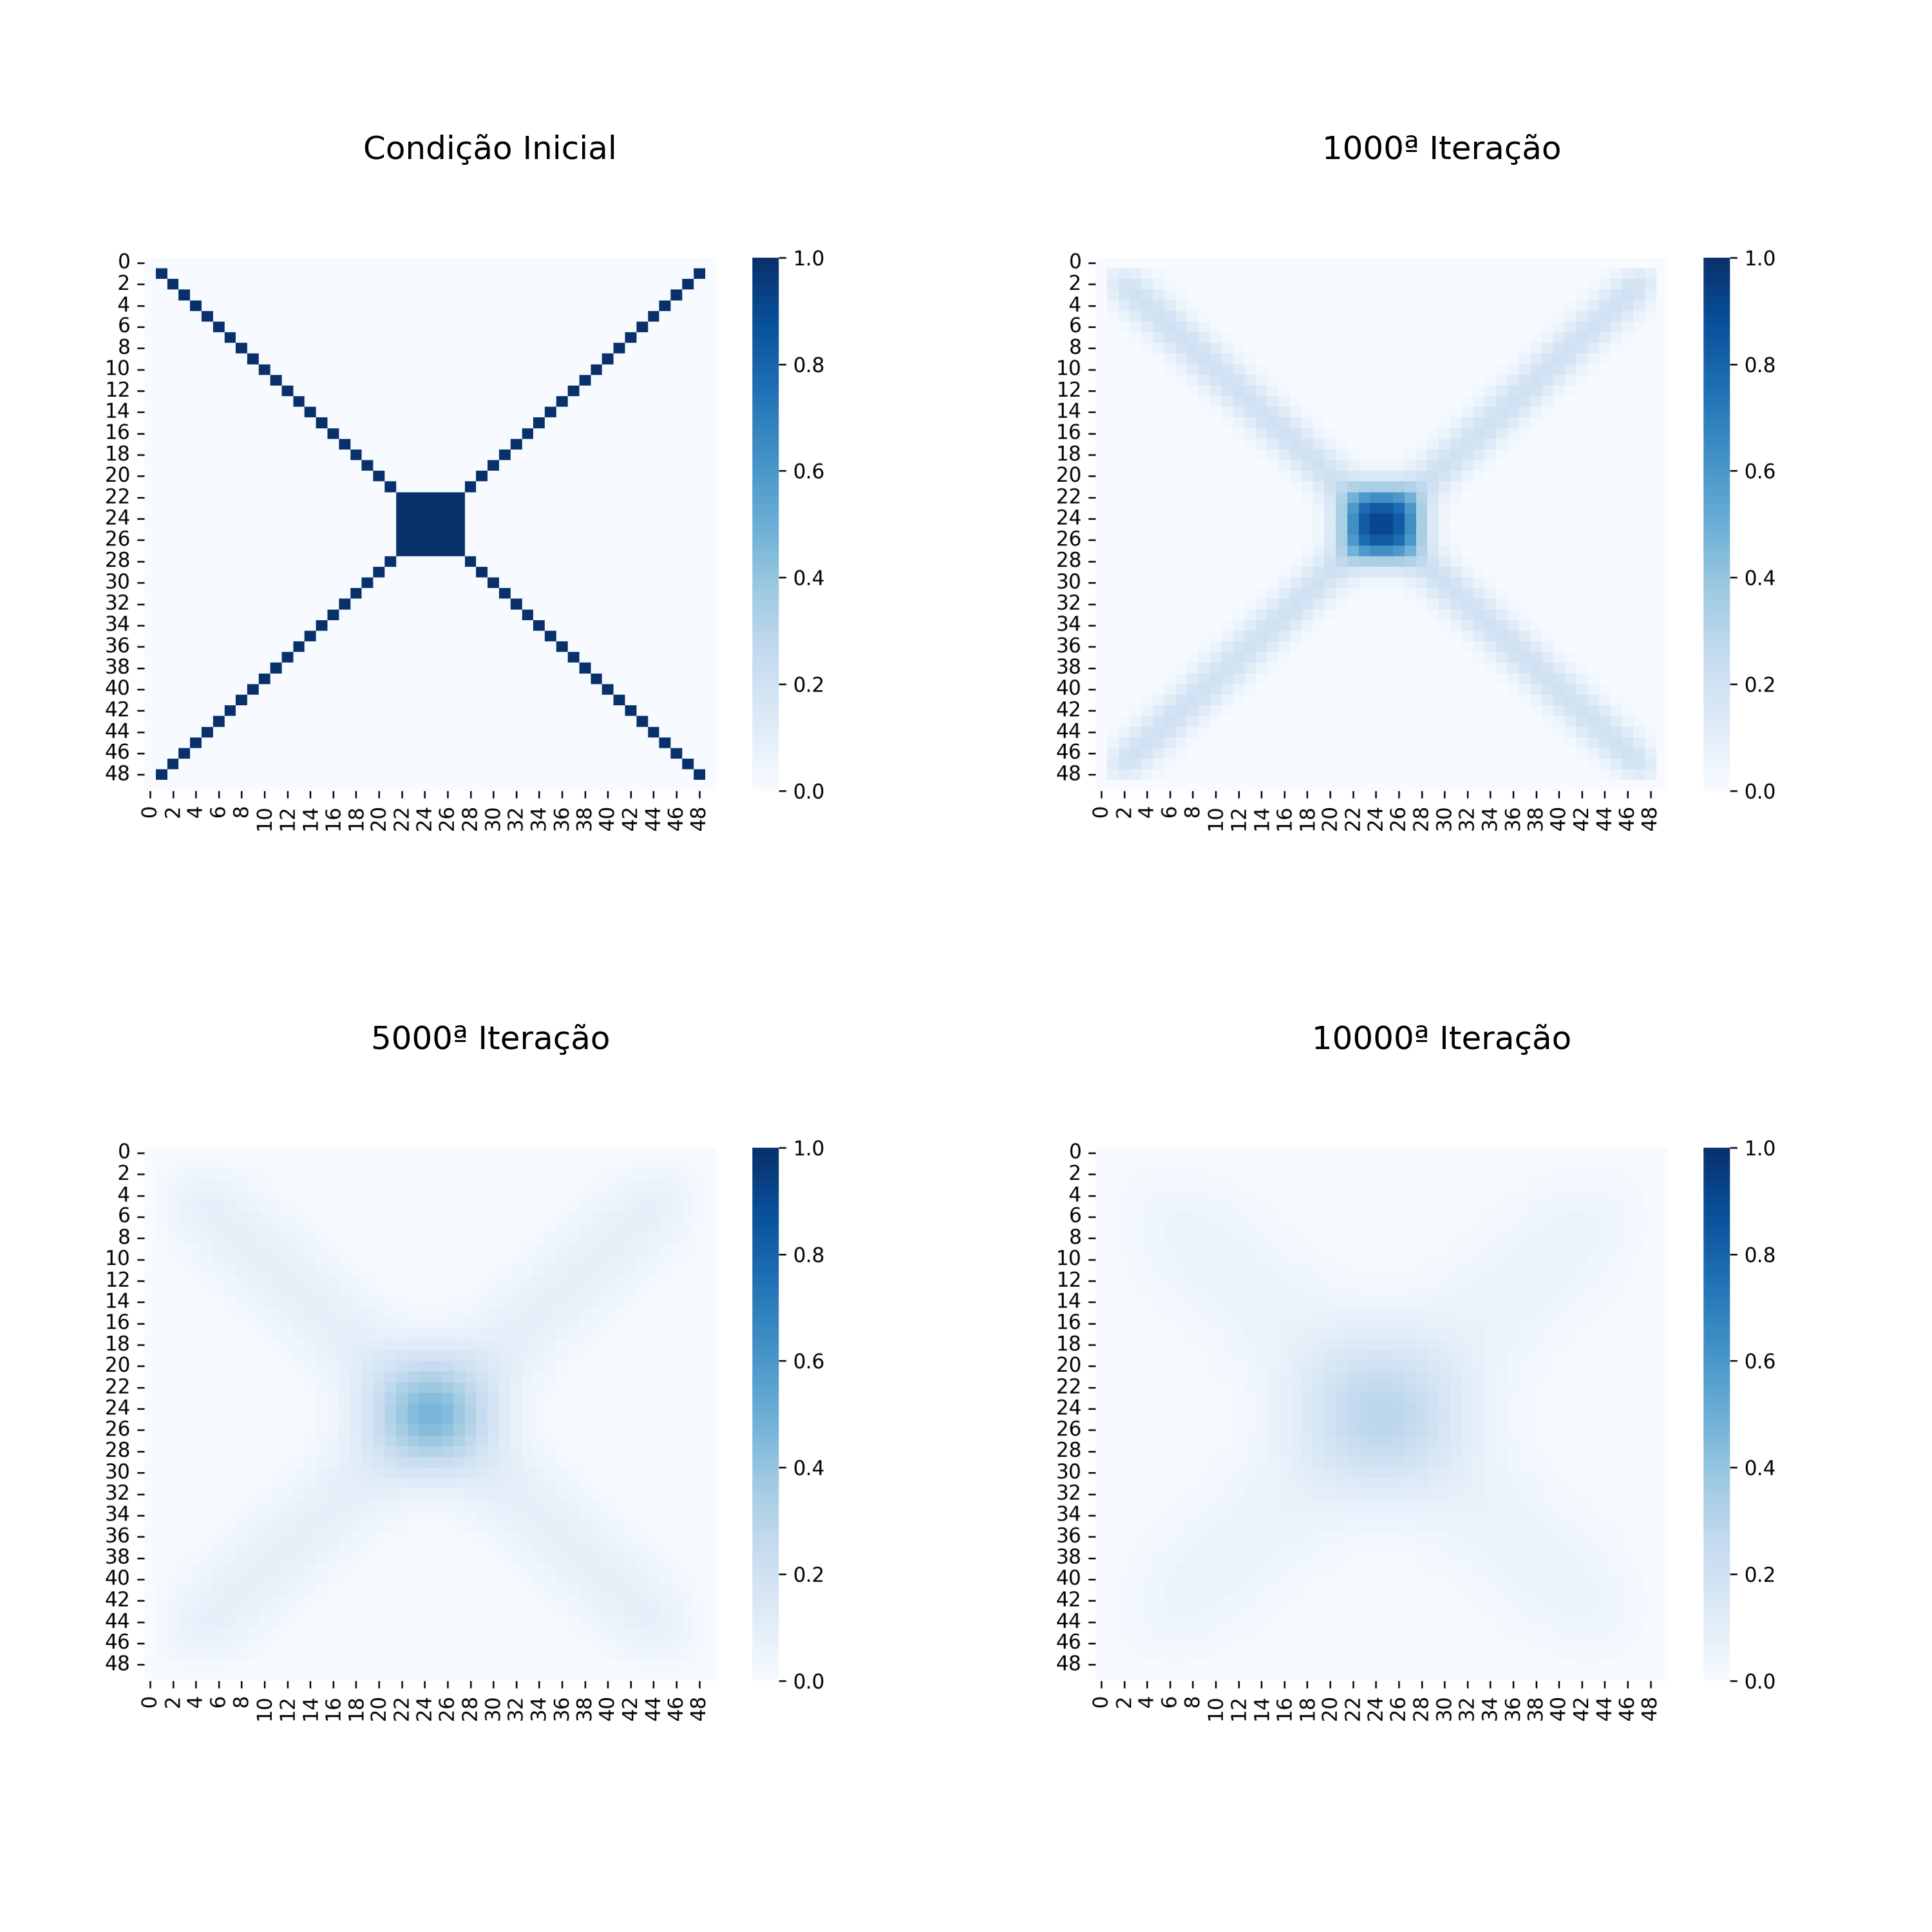
\includegraphics[width=.55\textwidth]{figs/heatmap.png}
  \caption{Mapa de calor em quatro instantes distintos da simulação.}
  \label{fig:heatmap}
\end{figure}

Analisando a progressão dos mapas de calor, observamos que o comportamento faz
sentido no contexto da solução proposta. Inicialmente, o contaminante é
adicionado com alta concentração nas diagonais e no centro da matriz,
evidenciado pelas regiões azuis escuros. Com o avanço das iterações, o
contaminante começa a se difundir para as regiões adjacentes, aumentando
gradativamente a luminosidade nessas áreas e diminuindo nos pontos de
concentração inicial. Na última iteração, a concentração se distribui
uniformemente pela matriz, com valores próximos entre si.

\subsection{Análise de Desempenho}

A análise de desempenho foi realizada em um computador \textit{desktop} com as
especificações apresentadas na Tabela~\ref{tab:especificacaoHardware}. Ademais,
as especificações dos parâmetros do problema foram incluídas na
Tabela~\ref{tab:especificacaoSimulacao}. Note que a simulação do código MPI foi
executada com variações no número de threads, porém mantendo em apenas uma
única thread OMP.

\begin{table}[ht]
  \centering
  \caption{Tabela de especificação de Hardware}
  \vspace{0.3cm}
  \begin{tabular}{||c c||}
    \hline
    Especificações      & Detalhes                  \\ [0.5ex]
    \hline\hline
    Processador         & Intel i7--4790 @ 3.60GHz  \\
    \hline
    Núcleos / Lógicos   & 4 / 8                     \\
    \hline
    Memória RAM         & 10 GB                     \\
    \hline
    Sistema Operacional & Ubuntu 22.04.05 (via WSL) \\
    \hline
  \end{tabular}
  \label{tab:especificacaoHardware}
\end{table}

\begin{table}[ht]
  \centering
  \caption{Tabela de especificação da Simulação}\label{tab:especificacaoSimulacao}
  \vspace{0.3cm}
  \begin{tabular}{||c c||}
    \hline
    Especificações             & Detalhes                    \\ [0.5ex]
    \hline\hline
    Dimensão da Matriz (N x N) & 2000 x 2000                 \\
    \hline
    Número de Iterações        & 500                         \\
    \hline
    Distribuição Inicial       & Alta concentração no centro \\
    \hline
    Coeficiente de Difusão     & 0.1                         \\
    \hline
    $\Delta t$                 & 0.01                        \\
    \hline
    $\Delta x$                 & 1.0                         \\
    \hline
  \end{tabular}
\end{table}

Para obter valores mais consistentes e minimizar influências externas, como
outros programas em execução, cada teste foi executado quinze vezes e, assim,
calculamos o tempo médio gasto e seu desvio padrão. O \textit{speedup} é
calculado dividindo-se o tempo de execução sequencial pelo tempo de execução
CUDA correspondente.

\begin{table}[ht]
  \centering
  \caption{Tabela de comparação de desempenho entre o código sequencial e o
    utilizando MPI.}\label{tab:results}
  \vspace{0.3cm}
  \begin{tabular}{||c c c c||}
    \hline
    Experimento  & N° Threads/Processos & Tempo             & SpeedUp \\ [0.5ex]
    \hline\hline
    Sequencial   & 1 T                  & 124.10 $\pm$ 0.73 & 1.0     \\
    \hline
    OMP          & 4 T                  & 12.28 $\pm$ 1.30  & 2.15     \\
    \hline
    CUDA (16x16) & ---                  & 5.04 $\pm$ 1.02   & 5.24     \\
    \hline
    MPI          & 1T/1P                & 25.39 $\pm$ 1.19  & 1.04    \\
    \hline
    MPI          & 1T/2P                & 15.67 $\pm$ 1.52  & 1.69    \\
    \hline
    MPI          & 1T/4P                & 14.14 $\pm$ 1.33  & 2.01    \\
    \hline
    MPI          & 1T/8P                & 15.52 $\pm$ 1.34  & 1.70    \\
    \hline
    MPI          & 1T/16P               & 16.83 $\pm$ 1.31  & 1.57    \\
    \hline
    MPI          & 1T/32P               & 20.19 $\pm$ 1.81  & 1.31    \\
    \hline
  \end{tabular}
\end{table}

O desempenho superior das aplicações com MPI em comparação com o sequencial se
deve ao fato de que, enquanto a execução sequencial processa todas as tarefas
de forma linear, o MPI divide a carga de trabalho entre vários processos que
operam simultaneamente. Isso reduz significativamente o tempo de execução,
especialmente para tarefas que podem ser facilmente paralelizadas, ao passo que
a execução sequencial enfrenta limitações de desempenho por processar tudo de
forma isolada, sem aproveitar o paralelismo.

\begin{figure}[H]
  \centering
  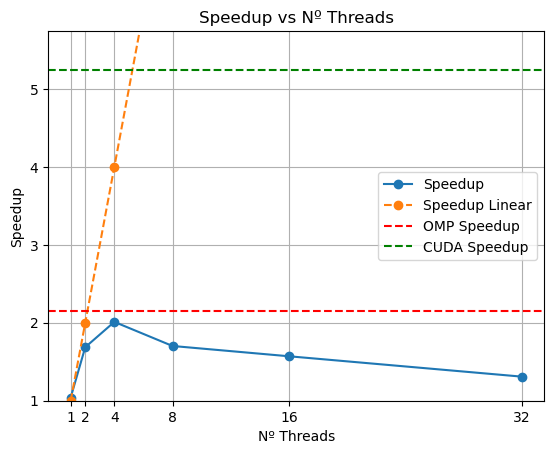
\includegraphics[width=.5\textwidth]{figs/speedupxthreads_MPI.png}
  \caption{Gráfico de comparação de speedup pelo numero de threads}
  \label{fig:speedupxthreads}
\end{figure}

A Figura~\ref{fig:speedupxthreads} ilustra os resultados do speedup encontrados
na Tabela~\ref{tab:results}. O melhor desempenho MPI é alcançado com 4
processos, enquanto configurações com 16 e 32 processos mostram redução no
speedup devido ao aumento do overhead de comunicação. As linhas horizontais
destacam o desempenho superior de OMP e, especialmente, CUDA, que aproveita
melhor o paralelismo em GPUs.

\section{Conclusão}
O uso de paralelismo com MPI proporciona ganhos significativos de desempenho em
relação à execução sequencial, especialmente com um número moderado de
processos, como 4, onde o balanceamento entre carga computacional e overhead é
mais eficiente. No entanto, o desempenho tende a decrescer com o aumento
excessivo de processos devido ao aumento do overhead de comunicação e
sincronização entre eles. Comparando com OMP e CUDA, é evidente que essas
tecnologias apresentam melhor eficiência para tarefas com alta demanda de
paralelismo, considerando o ambiente de execução em um computador doméstico com
GPU dedicada. Caso contrário, em um ambiente como um \textit{cluster} de
computadores, MPI seria a melhor opção para distribuir a carga de trabalho
entre os nós.

\bibliographystyle{sbc}
\bibliography{sbc-template}
\nocite{*}
\end{document}